\documentclass[a4paper]{scrartcl}

\usepackage[
fancytheorems, 
fancyproofs, 
noindent, 
%  spacingfix,  
]{adam}

\usepackage{tikz}
\usetikzlibrary{automata, positioning}

\title{Markov Chains}
\author{Adam Kelly (\texttt{ak2316@cam.ac.uk})}
\date{\today}


\allowdisplaybreaks

\begin{document}

\maketitle

A stochastic process is said to have the `Markov property' if, conditional on its present value, the future is independent of the past.
This is a \emph{restrictive} assumption, but we do end up with a useful model with a rich mathematical theory, which we shall study in this course.

This article constitutes my notes for the `Markov Chains' course, held in Michaelmas 2021 at Cambridge. These notes are \emph{not a transcription of the lectures}, and differ significantly in quite a few areas. Still, all lectured material should be covered.


\tableofcontents

% \clearpage

\section{The Markov Property}

\subsection{What is a Markov Chain?}

Let $S$ be a countable set (the set of possible `states'), and let $X_n$ be a sequence of random variables taking values in $S$.

\begin{definition}[Markov Chain]
	The sequence of random variables $X_n$ is a \vocab{Markov chain} if it satisfies the \vocab{Markov property}
	$$
	\PP(X_{n + 1} = x_{n + 1} \mid X_n = x_n, \dots, X_0 = x_0) = \PP(X_{n + 1} = x_{n + 1} \mid X_n = x_n).
	$$

	The Markov chain is said to be \vocab{homogeneous} if for all $i, j \in S$ the conditional probability $\PP(X_{n + 1} = j \mid X_n = i)$ is independent of $n$.
\end{definition}

In this course we are only going to study homogeneous Markov chains.

Markov chains are often best described by diagrams\footnote{You might notice that these diagrams are labelled directed graphs, and indeed you will see concepts from graph theory such as connectivity reoccur when we later talk about communicating classes.} which show the probability of moving from one state to another.
For example, the Markov chain in the diagram below has three states which we label $\{1, 2, 3\}$, and the probability of moving from state 1 to state 2 is $1/2$, and the probability of moving from state 2 to state 3 is $1/3$, and so on.

\begin{center}
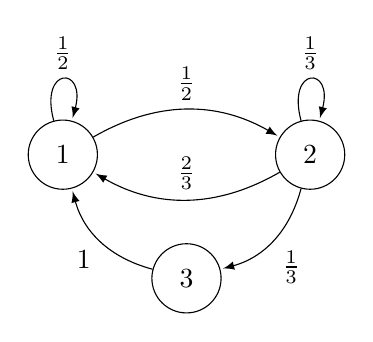
\begin{tikzpicture}

\node[state] (1) {1};
\node [right=of 1] (4) {};
\node[state, right=of 4] (2) {2};
\node[state, below=of 4] (3) {3};

\draw[every loop, >=latex]
(1) edge[loop above] node {$\frac{1}{2}$} (1)
(1) edge[bend left, auto=left] node {$\frac{1}{2}$} (2)
(2) edge[bend left, auto=left] node[above] {$\frac{2}{3}$} (1)
(2) edge[loop above] node {$\frac{1}{3}$} (2)
(2) edge[bend left, auto=left] node {$\frac{1}{3}$} (3)
(3) edge[bend left, auto=left] node {$1$} (1);

\end{tikzpicture}
\end{center}

In general, to calculate the probabilities associated with a Markov chain, we need to know two quantities.

\begin{itemize}
	\item \emph{The initial distribution}. We first need to know about the starting state of a Markov chain. This is described by the initial distribution $\lambda = (\lambda_i \mid i \in S)$, where $\lambda_i = \PP(X_0 = i)$.
	\item \emph{The transition probabilities}. We also need to know the probability of moving from a state $i \in S$ to a state $j \in S$. This is typically given by a \emph{transition matrix} $P = (P_{i, j} \mid i, j \in S)$ with $p_{i,j} = \PP(X_1 = j \mid X_0 = i)$.
\end{itemize}
These quantities are of course subject to some constraints, in that we require $\sum_{i \in S} \lambda_i = 1$ and the transition matrix $P$ must be \vocab{stochastic}, in that $\sum_{j \in S} P_{i, j} = 1$ for all $i \in S$.

If a Markov chain $X_n$ has initial distribution $\lambda$ and transition matrix $P$, we say that it is \vocab{$\markov(\lambda, P)$}.

Once we have these quantities, we can begin to actually establish various properties about the Markov chain, for example the probability that it goes through a given sequence of states.

\begin{theorem}[Probability of a Sequence of States]
	The sequence of random variables $X_n$ is $\markov(\lambda, P)$ if and only if
	$$
	\PP(X_0 = i_0, X_1 = i_1, \dots, X_n = i_n) = \lambda_{i_0}P_{i_0, i_1} \cdots P_{i_{n - 1}, i_n},
	$$
	for all $n \geq 0$ and $i_0, \dots, i_n \in S$.
\end{theorem}
\begin{proof}
	Let $A_k$ denote the event $\{X_k = i_k\}$. First suppose that $X_n$ is $\markov(\lambda, P)$. We prove the result holds by induction. For $n = 0$ this is true by definition. Then if it holds up to $n$, we have
	\begin{align*}
	\PP(A_0 \cap \cdots \cap A_n)  &= \PP(A_0 \cap \cdots \cap A_{n - 1})\PP(A_n \mid A_0 \cap \cdots \cap A_{n - 1}) \\
	&= \PP(A_0 \cap \cdots \cap A_{n - 1})\PP(A_n \mid A_{n - 1}) \\ 
	&= \left(\lambda_{i_0}P_{i_0, i_1} \cdots P_{i_{n - 2}, i_{n - 1}}\right)P_{i_{n - 1}, i_n},
\end{align*}
which completes our induction.

Conversely, suppose that the result holds. Then with $n = 0$ we get that the initial distribution of $X_n$ is $\lambda$. Then
$$
\PP(A_{n + 1} \mid A_{0} \cap \cdots \cap A_n) = \frac{\PP(A_0 \cap \cdots \cap A_{n + 1})}{\PP(A_0 \cap \cdots \cap A_{n})} = P_{i_{n}, i_{n + 1}}.
$$
Since this does not depend on $i_0, \dots, i_{n - 1}$, $X_n$ is a homogeneous Markov chain with transition matrix $P$, as required.
\end{proof}

\subsection{Simple Markov Property}

An important aspect of Markov chains is that they are \emph{memoryless}, in the future is independent of the past, conditional on the present. This is encapsulated in the \vocab{simple Markov property}.

\begin{theorem}[Simple Markov Property]
	Let $X_n$ be a Markov chain. Then conditional on $X_m = i$, the sequence of random variables $(X_{m + n})_{n \geq 0}$ is\footnote{Here $\delta_{ij}$ is 1 if $i = j$ and 0 otherwise.} $\markov(\delta_i, P)$, and is independent of $X_0, \dots, X_{m - 1}$.
\end{theorem}
\begin{proof}
	Given any event $H$ determined by $X_0, \dots, X_{m - 1}$, we want to show that for an event $F = \{X_m = i_m, \dots X_{m + n} = i_{m +n}\}$ we have
	$$
	\PP(H \cap F \mid X_m = i) = \delta_{ii_m}P_{i_m, i_{m + 1}} \cdots P_{i_{m + n-1}, i_{m + n}} \PP(H \mid X_m = i).
	$$
	Indeed, considering the case of $H = \{X_0 = i_0, \dots, X_m = i_m\}$ we have
	\begin{align*}
		\PP(H \cap F \mid X_m = i) &= \frac{\lambda_{i_0}P_{i_0, i_1} \cdots P_{i_{m - 1}, i}P_{i, i_{m + 1}} \cdots P_{i_{m + n - 1}, i_{m + n}}}{\PP(X_m = i)} \\
		&= \delta_{i i_m}P_{i, i_{m + 1}} \cdots P_{i_{m + n - 1}, i_{m + n}} \PP(H \mid X_m = i),
	\end{align*}
	as required. 
	
	Then for a general $H$, we can write it as the disjoint union $H = \bigcup_{k = 1}^{\infty} H_k$, and then the overall result follows by summing the above result for relevant $H_k$.
\end{proof}

\subsection{Transition Probabilities}

We are now going to address how to find the probability that a Markov chain is in a given state after $n$ steps.
The core idea of this section is that we will be able to reduce such questions into questions about the transition matrix that we introduced earlier.

Recall that if $X_n$ is a Markov chain with transition matrix $P$, then $P_{i, j}$ was the probability of moving from the state $i$ to the state $j$. We call these the \vocab{one-step transition probabilities}. We can generalize this slightly.

\begin{definition}[$n$-Step Transition Probabilities]
	For a Markov chain $X_n$, the \vocab{$n$-step transition probabilities} are given by
	$$
	p_{i, j}(n) = \PP(X_n = j \mid X_0 = i).
	$$
\end{definition}

These $n$-step transition probabilities naturally form the \vocab{$n$-step transition matrix} $P(n) = (p_{i, j}(n) \mid i, j \in S)$. The nice thing about writing these transition probabilities as a matrix is that they satisfy a lovely set of equations that relate extremely well to matrix algebra.

\begin{theorem}[Chapman-Kolmogorov Equations]
	We have that
	$$
	p_{i, j}(n + m) = \sum_{k \in S} p_{i, k}(n)p_{k, j}(m),
	$$
	where $i, j \in S$ and $m, n \geq 0$. In particular, $P(m + n) = P(m)P(n)$.
\end{theorem}
\begin{proof}
	Using the partition theorem and simple Markov property,
	\begin{align*}
		p_{i, j}(n + m) &= \PP(X_{n + m} = j \mid X_0 = i) \\
		&= \sum_{k \in S} \PP(X_{m + n} = j \mid X_n = k, X_0 = i) \PP(X_n = k \mid X_0 = i) \\
		&= \sum_{k \in S} \PP(X_{m + n} = j \mid X_n = k) \PP(X_n = k \mid X_0 = i) \\
		&= \sum_{k \in S} p_{i, k}(n) p_{k, j}(m).
	\end{align*}
\end{proof}

So, if we have some $n$-step transition matrix $P(n)$, the above result shows us that it satisfies $P(n) = P^n$. This reduces our problem to just this:

\begin{center}
	\color{blue}
	To compute $p_{i, j}(n)$, we can compute powers of\\ the transition matrix, and take $(P^n)_{i, j}$.
\end{center}

In general, this makes our problem significantly easier, and if the state space is finite, we can use tools from linear algebra such as diagonalisation.

\begin{example}[Computing Transition Probabilities]
	Let $\alpha, \beta \in (0, 1)$. 
	Consider the Markov chain $X_n$ with states $S = \{1, 2\}$, with transition matrix 
	$$
	P = \begin{pmatrix}
		1 - \alpha & \alpha \\
		\beta & 1 - \beta
	\end{pmatrix}.
	$$
	A diagram of this markov chain is shown below.
	\begin{center}
	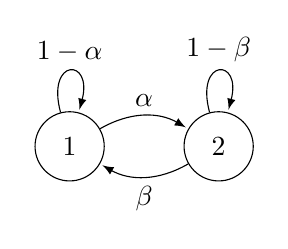
\begin{tikzpicture}

	\node[state] (1) {1};
	\node[state, right=of 1] (2) {2};

	\draw[every loop, >=latex]
	(1) edge[loop above] node {$1 - \alpha$} (1)
	(1) edge[bend left, auto=left] node {$\alpha$} (2)
	(2) edge[bend left, auto=left] node {$\beta$} (1)
	(2) edge[loop above] node {$1 -\beta$} (2);

	\end{tikzpicture}
	\end{center}

	We want to find the $n$-step transition probabilities.

	\textbf{Method 1} (Difference Equations). We are first going to find $p_{1, 1}(n)$ using a `bare-hands' method. By the Chapman-Kolmogorov equations (that is, conditioning on $X_n$) we have
	\begin{align*}
		p_{1, 1}(n + 1) &= p_{1, 1}(n)p_{1, 1}(1) + p_{1, 2}(n) p_{2, 1}(1) \\
		&= (1 - \alpha)p_{1, 1}(n) + \beta p_{1, 2}(n) \\
		&= (1 - \alpha)p_{1, 1}(n) + \beta (1 - p_{1, 1}(n)) \\
		&= p_{1, 1}(n)(1 - \alpha - \beta) + \beta.
	\end{align*}
	This is a recurrence relation which we can then solve using the boundary condition $p_{1, 1}(0) = 1$ to get
	$$
		p_{1, 1}(n) = \begin{cases}
			\frac{\alpha}{\alpha+\beta}+\frac{\alpha}{\alpha+\beta} \cdot(1-\alpha-\beta)^{n} &\mbox{if } \alpha + \beta > 0, \\
			1 &\mbox{if } \alpha + \beta = 0.
		   \end{cases}
	$$

	\textbf{Method 2} (Diagonalisation). An alternative solution uses some tools from matrix algebra. To calculate the $n$-step transition matrix $P^n$, we are going to diagonalise $P$.

	The eigenvalues of $P$ are given by the solutions to $\det(P - \mu I) = 0$, which are $\{1, 1 - \alpha - \beta\}$. Thus for some invertible matrix $U$ we have
	$$
	P = U^{-1}\begin{pmatrix}
		1 & 0 \\ 0 & 1 - \alpha - \beta
	\end{pmatrix}U \quad \text{and} \quad P^n = U^{-1} \begin{pmatrix}
		1 & 0 \\ 0 & (1 - \alpha - \beta)^n
	\end{pmatrix}U.
	$$
	Thus $p_{1, 1}(n) = A + B(1 - \alpha - \beta)^n$, for constants $A$ and $B$. We can find these by noting the boundary conditions $p_{1, 1}(0) = 1$ and $p_{1, 1}(1) = 1 - \alpha$, giving 
	$$
		p_{1, 1}(n) = \begin{cases}
			\frac{\alpha}{\alpha+\beta}+\frac{\alpha}{\alpha+\beta} \cdot(1-\alpha-\beta)^{n} &\mbox{if } \alpha + \beta > 0, \\
			1 &\mbox{if } \alpha + \beta = 0.
		   \end{cases}
	$$
\end{example}

In general, if the state space of a Markov chain is finite with $|S| = k$, then $P$ is a $k \times k$ matrix with eigenvalues $\mu_1, \dots, \mu_k$.

If \emph{all of the eigenvalues are distinct}, then $P$ is diagonalisable, and we can write
$$
P = U^{-1} \begin{pmatrix}
	\mu_1 & \cdots & 0 \\
	0 & \ddots & 0 \\
	0 & \cdots & \mu_k
\end{pmatrix} U \quad \text{and} \quad P^n = U^{-1} \begin{pmatrix}
	\mu_1^n & \cdots & 0 \\
	0 & \ddots & 0 \\
	0 & \cdots & \mu_k^n
\end{pmatrix} U,
$$
and $p_{i,j} = a_1 \mu_1^n + \cdots + a_k \mu_k^n$, for some constants $a_1, \dots, a_k$, which are determined by the boundary conditions.

If some eigenvalue $\mu_k$ is complex, then it's conjugate is also an eigenvalue, so if $\mu_k = re^{i \theta}$ we have also the eigenvalue $\overline{\mu_k} = re^{-i \theta}$, and we can write
$$
p_{i, j} = a_1 \mu_1^n + \cdots + a_{k - 2}\mu_{k - 2}^n + a_{k - 1}r^n \cos(n \theta) + a_k r^n \sin (n \theta),
$$
since $p_{i, j}$ is real and so all of the imaginary parts must cancel out.


If \emph{some eigenvalues repeat}, then the situation is slightly more complicated. If an eigenvalue $\mu_k$ has multiplicity $m$, we can simply replace $a_k$ by a degree $m$ polynomial in $n$\footnote{This comes from considering the Jordan Normal form of the transition matrix.}. 


\begin{example}[Transition Matrix with Complex Eigenvalues]
	Consider the markov chain $X_s$ with states $S = \{1, 2, 3\}$ as shown in the diagram below. We want to find the $n$-step transition probability $p_{i, i}(n)$.
	\begin{center}
	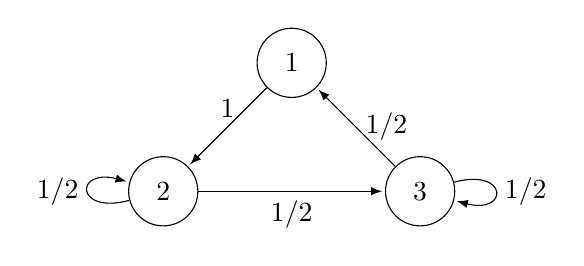
\begin{tikzpicture}

	\node[state] (1) {1};
	\node[state, below left=of 1] (2) {2};
	\node[state, below right=of 1] (3) {3};

	\draw[every loop, >=latex]
	(1) edge[above] node {$1$} (2)
	(2) edge[loop left] node {$1/2$} (2)
	(2) edge[below] node {$1/2$} (3)
	(3) edge[loop right] node {$1/2$} (3)
	(3) edge[right] node {$1/2$} (1);

	\end{tikzpicture}
	\end{center}

	This Markov chain has the transition matrix
	$$
	P = \begin{pmatrix}
		0 & 1 & 0 \\
		0 & 1/2 & 1/2 \\ 
		1/2 & 0 & 1/2
	\end{pmatrix},
	$$
	which has distinct eigenvalues $\{1, i/2, -i/2\}$.

	We can rewrite the complex eigenvalues using trigonometric functions as
	\begin{align*}
		\frac{i}{2} &= \cos \frac{\pi}{2} + i \sin \frac{\pi}{2}, \\ 
		-\frac{i}{2} &= \cos \frac{\pi}{2} - i \sin \frac{\pi}{2}.
	\end{align*}

	The general form for $p_{1,1}(n)$ is then given by
	$$
	p_{1n1}(n) = A + B \cdot \left(\frac{1}{2}\right)^n \cos \left(\frac{n \pi}{2}\right) + C \cdot \left(\frac{1}{2}\right)^n \sin\left(\frac{n \pi}{2}\right).
	$$
	The boundary conditions can be computed by hand as
	$p_{1,1}(0) = 1$, $p_{1,1}(1) = 0$ and $p_{1,1}(2) = 0$. This allows us to solve for $A$, $B$ and $C$ to get
	$$
	p_{1,1}(n) = \frac{1}{5} + \left(\frac{1}{2}\right)^n \left(\frac{4}{5}\cos\left(\frac{n \pi}{2}\right) - \frac{2}{5} \sin \left(\frac{n \pi}{2}\right)\right).
	$$
\end{example}

\section{Class Structure}


\subsection{Communicating Classes}

In Graph Theory, one can often make a problem easier by looking at the \emph{connected components} of the graph, effectively splitting it up into smaller disconnected chunks which are easier to understand on their own. 
This has a natural analogue in the study of Markov chains,\footnote{Indeed, one can view a Markov chain as a labelled directed graph, and then apply the same connected components argument to obtain the theory shown here.} where we consider which states can interact.

\begin{definition}[Communication]
	Let $X_n$ be a Markov chain. For $i, j \in S$, we say that $i$ \vocab{leads to} $j$, written $i \rightarrow j$, if $p_{i, j}(n) > 0$ for some $n \geq 0$.

	If $i \rightarrow j$ and $j \rightarrow i$, we say that $i$ and $j$ \vocab{communicate}, and write $i \leftrightarrow j$.
\end{definition}

We can use this idea of communication to break up our state space by noting that communication is an equivalence relation.

\begin{theorem}[Communication is an Equivalence Relation]
The relation $\leftrightarrow$ is an equivalence relation on $S$.
\end{theorem}
\begin{proof}
	For any $i \in S$, $p_{i, i}(0) = 1$ and thus $i \leftrightarrow i$, so the relation is reflexive. The relation is symmetric by definition, so we are just left to check transitivity.

	Let $i, j, k \in S$, and suppose that $i \leftrightarrow j$ and $k \leftrightarrow k$. Then there exists $m, n \geq 0$ such that $p_{i, j}(n) > 0$ and $p_{j, k}(m) > 0$. Then by the Chapman-Kolmogorov equations,
	\begin{align*}
		p_{i, k}(m + n) = \sum_{l \in S}p_{i, l}(m)p_{l, k}(n) \geq p_{i, j}(n) p_{j, k}(m) > 0,
	\end{align*}
	so $i \rightarrow k$. By the same argument $k \rightarrow i$, and thus $\leftrightarrow$ is transitive.
\end{proof}

Because communication is an equivalence relation, it partitions the state space.

\begin{definition}[Communicating Classes]
	The equivalence classes induced by $\longleftrightarrow$ on $S$ are called \vocab{communicating classes}.
\end{definition}

Because communication is really a notion about directed graphs (and not \emph{really} about individual probabilities), it's usually relatively easy to identify the communicating classes from the diagram of a Markov chain.

For example, the Markov chain below has its communicating classes coloured (and the transition probabilities are not labelled, as they are not needed to infer the communicating classes, aside from knowing they are non-zero along each edge).

\begin{center}
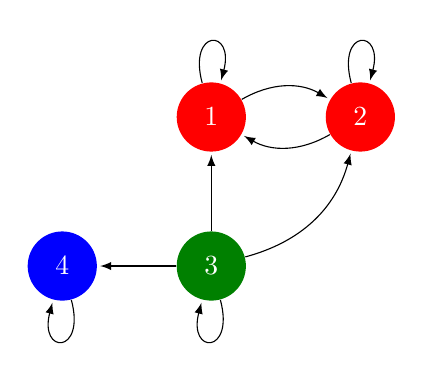
\begin{tikzpicture}

\tikzstyle{every state}=[fill,draw=none,blue,text=white]
\tikzstyle{accepting}=[green!50!black,text=white]
\tikzstyle{initial}= [red,text=white]

\node[state, initial] (1) {1};
\node[state, initial, right=of 1] (2) {2};
\node[state, accepting, below=of 1] (3) {3};
\node[state, left=of 3] (4) {4};

\draw[every loop, >=latex]
(1) edge[loop above] (1)
(1) edge[bend left, above] (2)
(2) edge[loop above] (2)
(2) edge[bend left, below] (1)
(3) edge[left] (1)
(3) edge[below] (4)
(3) edge[bend right, right] (2)
(3) edge[loop below] (3)
(4) edge[loop below] (4);

\end{tikzpicture}
\end{center}

In the Markov chain above, we can see that there are a few different ways that communicating classes can appear.

A communicating class $C$ is \vocab{closed} if there is no way to leave it, in that if $i \in C$ and $i \rightarrow j$, then $j$ in $C$. For example, in the Markov chain above, the communicating class $\{1, 2\}$ is closed.

A state $i \in S$ is \vocab{absorbing} if there is no way to leave that state, that is, $\{i\}$ is a communicating class. In the Markov chain above, $4$ is absorbing.

If a Markov chain has only one communicating class, we call is \vocab{irreducible}, as we cannot split it into smaller parts in this way.

% A communicating class $C$ is \vocab{closed} if whenever $x \in C$ and $x \rightarrow y$ then $y \in C$.

% A matrix $P$ is called \vocab{irreducible} if it has a single communicating class, that is, for all $i, y \in I$ we have $x \leftrightarrow y$. 

% A state $x$ is called \vocab{absorbing} if $\{x\}$ is a closed class. 


\section{Hitting Times, Stopping Times and Absorption Probabilities}

\subsection{Hitting Times}

When studying Markov chains, a frequently occurring question is `\emph{how long does it take to reach a given state $i \in S$?}', a concept which we formulate as the \emph{hitting time}.

\begin{definition}[Hitting Time]
	Let $X_n$ be a Markov chain.
	The \vocab{hitting time} of some subset of states $A \subseteq S$ is the random variable $T_A$, which is the least $n$ for which $T_n \in A$. 
	In particular,
	$$
	T_A = \inf\{n \geq 0 \mid X_n \in A\},
	$$
	where this may be $\infty$ if $X_n \not \in A$ for all $n \geq 0$.
\end{definition}

In this section, we will also look some related quantities, such as the \emph{hitting probability} and \emph{mean hitting time}.

\begin{definition}[Hitting Probability]
	Let $X_n$ be a Markov chain, and let $A \subseteq S$ be some subset of states.
	The \vocab{hitting probability} $h^A_i$ of $A$ is the probability that $X_n$ eventually reaches a state in $A$, given $X_0 = i$. That is,
	$$
	h^A_i = \PP(T_A < \infty \mid X_0 = i),
	$$
	where $i \in S$.
\end{definition}

\begin{definition}[Mean Hitting Time]
	Let $X_n$ be a Markov chain, and let $A \subseteq S$ be some subset of states.
	The \vocab{mean hitting time} $k^A_i$ of $A$ is the expected number of steps taken for $X_n$ to reach a state in $A$, given $X_0 = i$. That is,
	$$
	k^A_i = \EE[T_A \mid X_0 = i],
	$$
	where $i \in S$. We note that this may be $\infty$.
\end{definition}

So how do we go about calculating these quantities? An intuitive way is to try and consider what happens as we move from one state to another, as we will see in the example below.

\begin{example}[Computing Hitting Probabilities and Mean Hitting Times]
	Consider the Markov chain in the diagram below.
	\begin{center}
		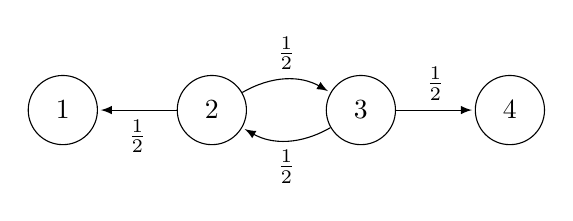
\begin{tikzpicture}
		
		\node[state] (1) {1};
		\node[state, right=of 1] (2) {2};
		\node[state, right=of 2] (3) {3};
		\node[state, right=of 3] (4) {4};
		
		\draw[every loop, >=latex]
		% (1) edge[loop above] node {1} (1)
		(2) edge[auto=left] node {$\frac{1}{2}$} (1)
		(2) edge[bend left, auto=left] node {$\frac{1}{2}$} (3)
		(3) edge[bend left, auto=left] node {$\frac{1}{2}$} (2)
		(3) edge[auto=left] node {$\frac{1}{2}$} (4);
		% (4) edge[loop above] node {1} (4);
		
		\end{tikzpicture}
		\end{center}

		Suppose we took $A = \{4\}$ and wanted to find the hitting probability $h_2^A = \PP(T_A < \infty \mid X_0 = 2)$. One might intuitively suppose that
		\begin{align*}
			h_2^A &= P_{2, 3} h_3^A = \frac{1}{2} h_3^A, \\
			h_3^A &= P_{3, 2} \cdot h_2^A + P_{3, 4} \cdot h_4^A = \frac{1}{2} \cdot h_2^A + \frac{1}{2}.
		\end{align*}
		which when solved gives us $h_2^A = 1/3$.

		Alternative, if we took $B = \{1, 4\}$ and wanted to find the mean hitting time $k_2^B$, we could again try the intuitive approach of writing
		$$
		k_2^B = 1 + \frac{1}{2}k_3^B,
		$$
		and noting that $k_3^B = k_2^B$ by symmetry, giving $k_2^B = 2$.
\end{example}

In the computations above, we really should check that these are valid methods (though it \emph{really is} quite intuitive).

\begin{theorem}[Computing Hitting Probabilities]
	Let $A \subseteq S$. Then the set of hitting probabilities $h^A = (h_i^A \mid i \in S)$ is the minimal\footnote{Minimal in that if $x$ is another non-negative solution, then $x_i \geq h_i^A$ for all $i \in S$.} non-negative solution to the equations
	\begin{align*}
		h_i^A = \begin{cases}
			1 &\mbox{if } i  \in A, \\
			\sum_{j \in S} P_{i, j} h_j^A &\mbox{if } i \not \in A.
		   \end{cases}
	\end{align*}
\end{theorem}
\begin{proof}
	We first check that $h_i$ solves this system. Clearly if $i \in A$, then $h_i^A = 1$, so take $i \in S\backslash A$. Then conditioning on the first step in the chain,
	\begin{align*}
		h_i^A &= \sum_{j \in S} P_{i, j} \PP(T_A < \infty \mid X_0 = i, X_1 = j)  \\
		&= \sum_{j \in S} P_{i, j} h_j^A,
	\end{align*}
	by the simple Markov property. So $h_i$ does indeed solve this system.

	We now check minimality. Let $x = (x_i \mid i \in S)$ be another non-negative solution. For $i \in A$, we have $x_i = h^A_i = 1$, so that holds. Then for $i \in S \backslash A$, since $x$ satisfies the system of equations we can write
	\begin{equation}\label{eq:1}
		x_i = \sum_{j \in S}P_{i, j} x_j = \sum_{j \in A} P_{i, j} x_j + \sum_{j \in S \backslash A} P_{i, j} x_j. \tag{$\dagger$}
	\end{equation}
	Then with $x_j = 1$ for $j \in A$ and $x \geq 0$, we have
	\begin{align*}
		x_i \geq \sum_{j \in A} P_{i, j} = \PP(X_1 \in A \mid X_0 = i) = \PP(T_A < 2 \mid X_0 = i).
	\end{align*}
	Similarily, expanding \eqref{eq:1}, we have
	\begin{align*}
	x_i &= \PP(X_1 \in A \mid X_0 = i) + \sum_{j \in S \backslash A} P_{i, j} \left(\sum_{k \in A} P_{j, k} x_k + \sum_{k \in S \backslash A} P_{j, k} x_k\right) \\
		&\geq \PP(X_1 \in A \mid X_0 = i) + \PP(X_1 \not \in A, X_2 \in A \mid X_0 = i) \\
		&= \PP(T_A < 3 \mid X_0 = 1).
	\end{align*}
	We can repeat this argument to eventually establish that $x_i \geq \PP(T_A < n \mid X_0 = i)$, for all $n \geq 0$. Then as $n \rightarrow \infty$, we have $x_i \geq \PP(T_A < \infty \mid X_0 = i)$, as required.
\end{proof}

This method of computing hitting probabilities is perfectly valid on Markov chains with infinite state spaces.

\begin{example}[Hitting Probabilities on an Infinite State Space]
	Consider the Markov chain with states $S = \{0, 1, \dots\}$ such that $P_{0, 1} = 1$, and
	$$
	P_{i, i+1} = p, \quad P_{i, i - 1} = q \quad \text{for all } i \geq 1,
	$$ 
	where $p, q \in (0, 1)$ with $p + q = 1$.

	\begin{center}
		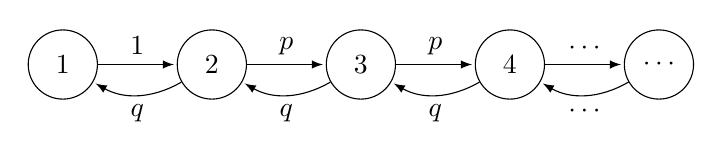
\begin{tikzpicture}
		
		\node[state] (1) {1};
		\node[state, right=of 1] (2) {2};
		\node[state, right=of 2] (3) {3};
		\node[state, right=of 3] (4) {4};
		\node[state, right=of 4] (5) {$\cdots$};
		
		\draw[every loop, >=latex]
		(1) edge[above] node {1} (2)
		(2) edge[above] node {$p$} (3)
		(3) edge[above] node {$p$} (4)
		(4) edge[above] node {$\cdots$} (5)
		(2) edge[bend left, below] node {$q$} (1)
		(3) edge[bend left, below] node {$q$} (2)
		(4) edge[bend left, below] node {$q$} (3)
		(5) edge[bend left, below] node {$\cdots$} (4);
		\end{tikzpicture}
		\end{center}

	Let $h_i = \PP(T_0 < \infty \mid X_0 = i)$, and suppose that $p \neq q$. Then we clearly have $h_0 = 1$, and generally we can write down the recurrence 
	$$
		h_i = p h_{i + 1} + qh_{i - 1}.
	$$
	This then implies $p(h_{i + 1} - h_i) = q(h_{i} - h_{i - 1})$, so that
	$$
		h_{i+1} - h_{i}  = \left(\frac{q}{p}\right)^i (h_1 - 1).
	$$
	This inspires us to write $h_i$ as a telescoping sum
	\begin{align*}
		h_i &= \sum_{j = 1}^i (h_j - h_{j - 1}) + 1  \\
			&= (h_1 - 1) \sum_{j = 1}^i \left(\frac{q}{p}\right)^j + 1,
	\end{align*}
	which gives us our general solution $h_i = a + b(q/p)^i$, which we can then solve.

	In the case that $q > p$, then in order for $h_i$ to be the minimal solution, we need to have $a = 1$ and $b = 0$, so $h_i = 1$.
\end{example}

% \begin{example}[Birth and Death Chains]
% 	Consider the Markov chain similar to before with states $S = \{0, 1, \dots\}$ such that $P_{0, 1} = 1$ and $P_{i, i + 1} = p$ 
% \end{example}

We also need to check that our method for calculating the mean hitting time was valid.

\begin{theorem}[Computing Mean Hitting Times]
	Let $A \subseteq S$. Then the set of mean hitting times $k^A = (k_i^A \mid i \in S)$ is the minimal non-negative solution to the equations
	\begin{align*}
		k_i^A = \begin{cases}
			0 &\mbox{if } i  \in A, \\
			1 + \sum_{j \in S\backslash A} P_{i, j} k_j^A &\mbox{if } i \not \in A.
		   \end{cases}
	\end{align*}
\end{theorem}
\begin{proof}
	We first check that $k_i$ solves this system. Clearly if $i \in A$, then $k_i^A = 0$, so take $i \in S \backslash A$. Then conditioning on the first step in the chain,
	\begin{align*}
		k_i^A &= \sum_{j \in S} P_{i, j}\EE[T_A \mid X_0 = i, X_1 = j]  \\
		&= \sum_{j \in S} P_{i, j}(1 + \EE[T_A \mid X_0 = j]) \\
		&= 1 + \sum_{j \in S} P_{i, j} k_j^A, 	
	\end{align*}
	which is equivalent to our original sum.

	We now show that the solution is minimal. Let $y = (x_i \mid i \in S)$ be another non-negative solution. Then for $i \in A$ we have $y_i = k_i^A = 0$, so consider $i \in S \backslash A$. We can then write
	\begin{align*}
	y_i &= 1 + \sum_{j \in S \backslash A} P_{i, j} y_j  \\
	&= 1 + \sum_{j \in S \backslash A} P_{i, j}\left(1 + \sum_{k \in S \backslash A} P_{j, k} y_k\right) \\
	&\geq \PP(T_A \geq 1 \mid X_0 = i) + \PP(T_A \geq 2 \mid X_0 = 1).
	\end{align*}
	By iterating this, we obtain
	$$
	y_i \geq \sum_{m = 1}^n \PP(T_A \geq m \mid X_0 = i),
	$$
	and taking the limit as $n \rightarrow \infty$, this gives
	$$
	y_i \geq \sum_{m = 1}^{\infty} \PP(T_A \geq m \mid X_0 = i) = k_i^A,
	$$
	where we note that for a random variable $M$ taking non-negative integer values we have $\EE[M] = \sum_{m = 1}^{\infty} \PP(M \geq m).$
\end{proof}

So it does work, how lovely.

\subsection{Stopping Times and the Strong Markov Property}

We previously proved the \emph{simple Markov property}, that 
conditional on the value of a Markov chain at a given time $m$, the future is independent of the past.
This property required that we take some fixed time $m$ -- but what if $m$ itself is random? It's \emph{not} true in general\footnote{For example, let $T$ be the first time that a Markov chain hits some value $i$. Then if we condition on time $T - 1$, the future is then determined since the next step will be to $i$! You will see that this type of event is not allowed in our definition of stopping times.} that the Markov property still holds for an arbitrary random time, but it is true for certain kinds of times.

\begin{definition}[Stopping Times]
	A random time $T : \Omega \rightarrow \{0, 1, \dots\} \cup \{\infty\}$ is a \vocab{stopping time} for a Markov chain $X_n$ if for all $n \geq 0$ the event $\{T = n\}$ is given in terms of $X_0, X_1, \dots, X_n$ only.
\end{definition}

In particular, random times that `look into the future' are not stopping times. A straightforward example of a stopping time is the hitting time $T^A$ that we defined in the previous section.

With stopping times, we can indeed make a statement similar to the Markov property using random times.

\begin{theorem}[Strong Markov Property]	
Let $X_n$ be a Markov chain with transition matrix $P$, and let $T$ be a stopping time. Then conditional on $T < \infty$ and $X_T = i$, the sequence of random variables $(X_{T + n})_{n \geq 0}$ is $\markov(\delta_i, P)$ and is independent of $X_0, \dots, X_T$.
\end{theorem}
\begin{proof}
Let $H$ be an event given in terms of $X_0, \dots, X_{T - 1}$. Then it suffices to show that
\begin{align*}
	&\ \PP(X_{T + 1} = i_1, \dots, X_{T + n} = i_n, H \mid T < \infty, X_T = i)  \\
	&= \PP(X_1 = i_1, \dots, X_n = i_n \mid X_0 = i) \PP(H \mid T < \infty, X_T = i).
\end{align*}
The event $H \cap \{T = m\}$ is given in terms of $X_1, X_2, \dots, X_m$ only. Furthermore, $X_T = X_m$ when $T = m$. We condition on the event $H \cap \{T = m\} \cap \{X_m = i\}$ and use the simple Markov property at time $m$ to get
\begin{align*}
&\ \PP(X_{T + 1} = i_1, \dots, X_{T + n} = i_n, H \mid T < \infty, X_T = i) \\
&= \PP(X_1 = i_1, \dots, X_n = i_n) \PP(H, T = m, X_T = i).
\end{align*}
Summing this over $m = 0, 1, \dots$ and dividing by $\PP(T < \infty, X_T = i)$ then gives the desired result.
\end{proof}

\subsection{Recurrence and Transience}

We now consider states that a Markov chain continues to come back to, or only visits finitely many times.

% Definition of Recurrennt and Transient

\begin{lemma}[Probability of Repeated Visiting]
	$\PP(V_i > r \mid X_0 = i) = f_i^r$, for all $r \in \N$.
\end{lemma}
\begin{proof}
	Suppose it is true for $r$. We need to show that
	\begin{align*}
		\PP(V_i > r + 1 \mid X_0 = i) &= \PP(T_i^{(r + 1)} < \infty \mid X_0 = i) = \PP(T_i^{(r + 1)} < \infty, T_i^{(r)} < \infty) \\
		&= \PP(T_i^{(r + 1)} < \infty \mid T_i^{(r)} < \infty, T_0 = i) \cdot \PP(T_i^{(r)} < \infty \mid X_0 = i) \\
		&= \PP(T_i^{(r + 1)} < \infty \mid T_i^{(r)} < \infty, T_0 = i) \cdot f_i^r. 
	\end{align*}
	By the strong Markov property applied to $T_i^{(r)}$ (which is a stopping time), we get
	$$
	\PP(T_i^{(r + 1)} < \infty \mid X_0 = i) = \PP(T_i < \infty \mid X_0 = i) = f_i,
	$$
	and thus our result holds.
\end{proof}

\begin{theorem}[Recurrence and Transience Criterion]
	Let $X_n$ be a markov chain with transition matrix $P$, and let $i \in S$. Then we have the following dichotomy:
	\begin{enumerate}[label=(\arabic*)]
		\item If $\PP(T_i< \infty \mid X_0 = i) = 1$, then $i$ is recurrent and $\sum_{n = 0}^{\infty} p_{i, i}(n)$ is infinite.
		\item If $\PP(T_i < \infty \mid X_0 = i) < 1$, then $i$ is transient and $\sum_{n = 0}^{\infty} p_{i, i}(n) < \infty$.
	\end{enumerate}
\end{theorem}
\begin{proof}
	We can write $V_i$ using indicator functions as
	$
	V_i = \sum_{n = 0}^{\infty} \ii[X_n = 1],
	$
	and then by linearity of expectation we can write
	$$
	\EE[V_i \mid X_0 = i] = \sum_{n = 0}^{\infty} \PP(X_m = i \mid X_0 = i) = \sum_{n = 0}^{\infty} p_{i, i}(n).
	$$
	
	\emph{Part (1)}. If $f_i = 1$, then for all $r$ we have $\PP(V_i > r \mid X_0 = i) = 1$, and thus $\PP(V_i = \infty \mid X_i = 0) = 1$, implying that $i$ is recurrent, and $\EE[V_i \mid X_0 = i] = \infty$, implying that $\sum_{n = 0}^{\infty} p_{i, i}(n) = \infty$.

	\emph{Part (2)}. If $f_i < 1$, then by the previous lemma we have $\EE[V_i \mid X_0 = i] = 1/(1 - f_i) < \infty$, implying that $\PP(V_i < \infty \mid X_0 = i) = 1$, so $i$ is transient, and $\sum_{n = 0}^{\infty} p_{i, i}(n)$.
\end{proof}

\begin{theorem}[Recurrence and Transience of Communicating States]
	Let $x$ and $y$ be two states that communicate. Then either they are both recurrent or they are both transient.
\end{theorem}
\begin{proof}
	Suppose that $x$ is recurrent. We will show that $y$ is also recurrent. Since $x \rightarrow y$, there is some $m, l \in \N$ such that $p_{x, y}(m) > 0$ and $p_{y, x}(l) > 0$. Then we know that $\sum_{n = 0}^{\infty} p_{x, x}(n) = \infty$, and then
	\begin{align*}
	\sum_{n = 0}^{\infty} p_{y, y}(n) 
	&\geq \sum_{n = 0}^{\infty} 
	p_{y, y}(n + m + l) \\ 
	&\geq \sum_{n = 0}^{\infty} p_{y, x}(l) p_{x, x}(n) p_{x, y}(m)  \\
	&\geq p_{y, x}(l) p_{x, y}(m) \sum_{n = 0}^{\infty} p_{x, x}(n) = \infty.
	\end{align*}
\end{proof}

This immediately can be applied to the entire class structure of a Markov chain.

\begin{corollary}[Class Structure of Recurrence and Transience]
	Either all of the states in a communicating class are recurrent or they are all transient.
\end{corollary}

Recurrent communicating classes have a certain flavour to them, which should be intuitive. Really, for a communicating class to be recurrent we have to avoid getting stuck outside of that given communicating class. This forces closure of the communicating class.

\begin{theorem}[Closure of Recurrent Communicating Classes]	
	If $C$ is a recurrent communicating class, then it must be closed.
\end{theorem}
\begin{proof}
	Suppose that $C$ was not closed. Then there exists $x \in C$ and $Y \not \in C$ such that $x \rightarrow y$. Let $n$ be such that $p_{x, y}(n) > 0$. If starting from $x$ we hit $y$ at some point, then we can never visit $x$ again so
	$$
	\PP(V_x < \infty \mid X_0 = x) \geq \PP(X_m = y \mid X_0 = x) = p_{x, y}(m) > 0,
	$$
	so $x$ is not current which is a contradiction.
\end{proof}

\begin{theorem}[Finite Closed Classes are Recurrent]
	A finite closed class is recurrent.
\end{theorem}
\begin{proof}[Proof Sketch]
	Pick any state $x$ in the class. By pigeonhole there's another recurrent state $y$ communicating with $x$. Then there's positive probability of moving from $x$ to $y$ and $y$ to $x$, and this implies that $x$ is also recurrent.
\end{proof}

\begin{theorem}
	Let $P$ be irreducible and recurrent. Then for all $x$ and $Y$, $\PP(T_y < \infty \mid X_0 = x) = 1$.
\end{theorem}
\begin{proof}
	Omitted.
\end{proof}

\begin{theorem}[Pólya]
	A simple random walk in $\Z^d$ is recurrent for $d = 1$ and $d = 2$ and transient for $d \geq 3$.
\end{theorem}

Said in a better way, a drunk man will find his way home, but a drunk bird may get lost forever.



\end{document}

